%! Author = melek
%! Date = 9.06.2022

% Preamble
\documentclass[11pt]{article}

% Packages
\usepackage{amsmath}
\DeclareMathOperator*{\argmax}{argmax}

\usepackage{graphicx}
\usepackage{amssymb}
\usepackage{bm}

\graphicspath{ {../images/} }


% Document
\begin{document}

    \maketitle
    \setcounter{section}{12}

    \section{Exercises}

    \subsection{Question}

    Use your knowledge of the gridworld and its dynamics to determine an exact symbolic expression for the optimal probability of selecting the right action in Example 13.1.

    \subsection*{Answer}

    \noindent By equation 13.2, probability selecting right action:

    \noindent $ \pi( a | s, \theta) = \frac{e^{h(s,a,\theta)}}{\sum_{b} e^{h(s,b,\theta)}} $

    \noindent $ \pi( right | s, \theta) = \frac{e^{h(s,right,\theta)}}{e^{h(s,right,\theta)} + e^{h(s,left,\theta)}} $

    \hfill \break
    \noindent Incorporating 13.3 and feature vectors:

    \noindent $ \pi( right | s, \theta) = \frac{e^{\theta^{T}[1,0]}}{e^{{\theta^{T}[1,0]}} + e^{\theta^{T}[0,1]}} = \frac{e^{\theta_{1}}}{e^{{\theta_{1}}} + e^{\theta_{2}}} $

    \hfill \break
    \noindent From example 3.1 we know that probability of selecting right action is 0.59 then one probable parameter vector can be $ \theta = [-0.53, -0.89] $:

    \subsection{Question}

    Generalize the box on page 199, the policy gradient theorem (13.5), the proof of the policy gradient theorem (page 325), and the steps leading to the REINFORCE update equation (13.8), so that (13.8) ends up with a factor of $ \gamma^t $ and thus aligns with the general algorithm given in the pseudocode.

    \subsection*{Answer}

    \noindent The text states in the boxed page 199: If there is discounting ( $\gamma < 1 $) it should be treated as a form of termination, which can be done simply by including a factor of $\gamma$ in the second term of 9.2.

    \noindent Equation 9.2 with discounting:

    \noindent $ \eta(s) = h(s) + \gamma \sum_{\bar{s}} \eta(\bar{s}) \sum_{a} \pi(a|\bar{s}) p(s| \bar{s},a)  $

    \hfill \break
    \noindent Proof of policy gradient theorem changes in the way $ \nabla v_{\pi}(s_0) $ is expanded:

    \noindent $ \nabla J(\theta) = \nabla V_{\pi}(s_{0})  $

    \noindent $ \nabla J(\theta) = \sum_{s} ( \sum_{k=0}^{\infty} \gamma^{k} \Pr(s_0 \rightarrow s, k, \pi )  ) \sum_{a} \nabla \pi(a|s) q_\pi (s,a) $

    \hfill \break
    \noindent I cannot show how $ \gamma^k $ is handled from here on.
    At the end the REINFORCE update 13.8 becomes:

    \noindent $ \theta_{t+1} = \theta{t} + \alpha \gamma^t G_{t} \frac{\nabla\pi(A_t | S_t , \theta_t)}{\pi(A_t | S_t , \theta_t)} $

    \hfill \break
    \noindent Alternative solution may be found in UCL leacture series.

     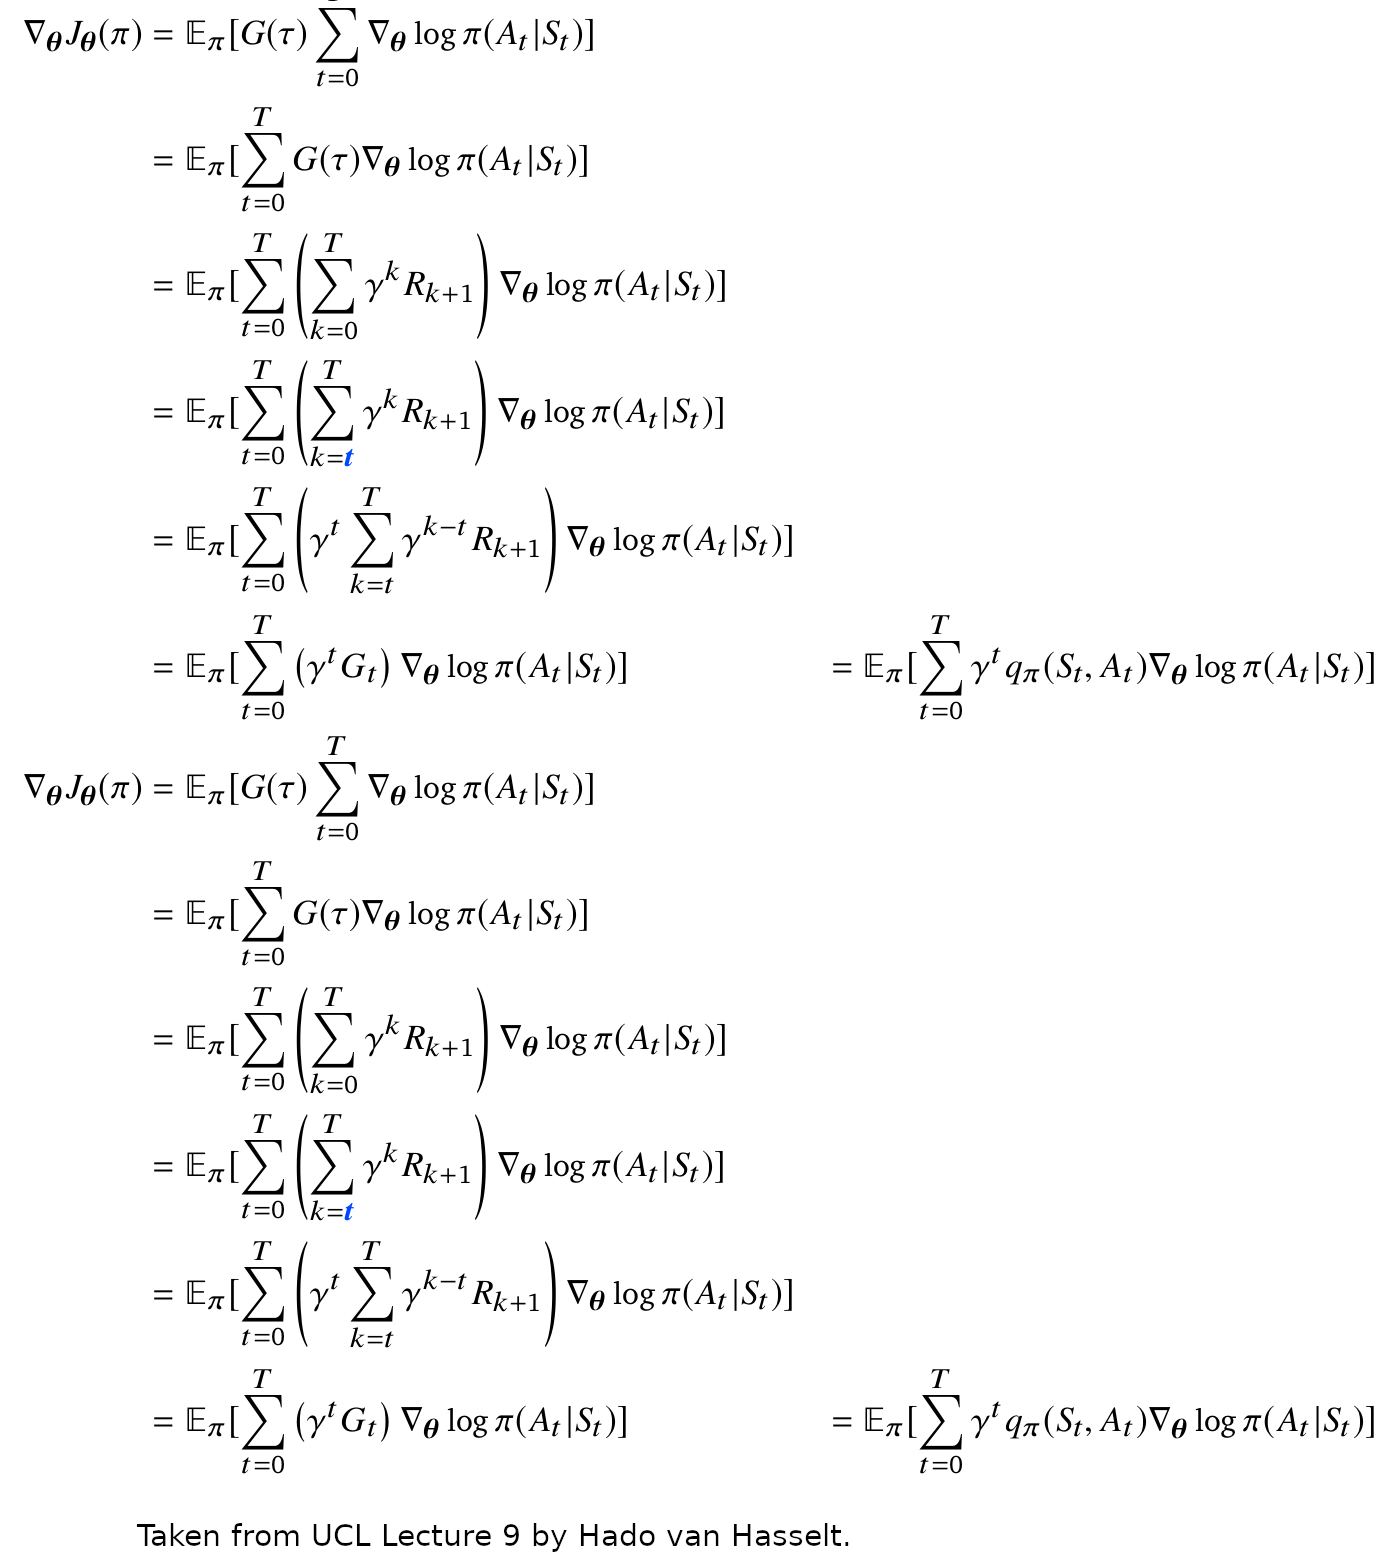
\includegraphics[scale=0.3]{exercise_13_3}

    \newpage
    \subsection{Question}

    In Section 13.1 we considered policy parameterizations using the soft-max in action preferences (13.2) with linear action preferences (13.3).
    For this parameterization,prove that the eligibility vector is:

    \hfill \break
    \noindent $ \nabla \ln \pi(a|s,\theta) = x(s,a) - \sum_{b} \pi(b|s,\theta) x(s,b)  $ \hfill (13.9)

    \hfill \break
    \noindent using the definitions and elementary calculus.

    \subsection*{Answer}

    \noindent Equation 13.2 is:

    \noindent $ \pi(a|s,\theta) = \frac{e^{h(s,a,\theta)}}{\sum_{b} e^{h(s,b,\theta)}} $

    \hfill \break
    \noindent Equation 13.3 is:

    \noindent $ h(s,a,\theta) = \theta^T x(s,a) $

    \hfill \break
    \noindent Let's start with 13.2 taking logarithm of both sides :

     \noindent $ \ln \pi(a|s,\theta) = \ln \frac{e^{h(s,a,\theta)}}{\sum_{b} e^{h(s,b,\theta)}} $

    \noindent $ \ln \pi(a|s,\theta) =  \ln  e^{h(s,a,\theta)} - \ln \sum_{b} e^{h(s,b,\theta)} $

    \noindent $ \ln \pi(a|s,\theta) =  h(s,a,\theta)  - \ln \sum_{b} e^{h(s,b,\theta)} $

     \hfill \break
    \noindent Now take derivative both sides :

     \noindent $ \nabla \ln \pi(a|s,\theta) =  \nabla h(s,a,\theta)  - \nabla  \ln \sum_{b} e^{h(s,b,\theta)} $

    \noindent $ \nabla \ln \pi(a|s,\theta) =  \nabla h(s,a,\theta)  -  \frac{\nabla  \sum_{b} e^{h(s,b,\theta)}}{\sum_{b} e^{h(s,b,\theta)}}  $

    \noindent $ \nabla \ln \pi(a|s,\theta) =  \nabla h(s,a,\theta)  -  \frac{  \sum_{b} \nabla e^{h(s,b,\theta)}}{\sum_{b} e^{h(s,b,\theta)}}  $

    \noindent $ \nabla \ln \pi(a|s,\theta) =  \nabla h(s,a,\theta)  -  \frac{  \sum_{b} \nabla h(s,b,\theta) e^{h(s,b,\theta)}}{\sum_{b} e^{h(s,b,\theta)}}  $

    \noindent $ \nabla \ln \pi(a|s,\theta) =  \nabla h(s,a,\theta)  -  \sum_{b} \nabla h(s,b,\theta) \pi(b|s,\theta)  $ from equation 13.2

    \noindent $ \nabla \ln \pi(a|s,\theta) =  x(s,a)  -  \sum_{b} x(s,b) \pi(b|s,\theta)  $ from equation 13.3


    \subsection{Question}

    Show that for the gaussian policy parameterization (13.19) the eligibility vector has the following two parts:

    \subsection*{Answer}

    \noindent Relevant equations are:

    \noindent $ \mu(s,\theta) = \theta_\mu x_\mu(s) $

    \noindent $ \sigma(s,\theta) = e^{\theta_{\sigma}^T x_\sigma(s)} $

    \hfill \break
    \noindent Taking logarithm of the policy function:

    \noindent $ \ln \pi(a|s,\theta) = \ln \frac{e^{- \frac{(a-\mu(s,\theta))^2}{2\sigma(s, \theta)^2}}}{\sigma(s,\theta)\sqrt{2\pi}}$

    \noindent $ \ln \pi(a|s,\theta) = \ln e^{- \frac{(a-\mu(s,\theta))^2}{2\sigma(s, \theta)^2}} -  \ln \sigma(s,\theta)\sqrt{2\pi}$

    \noindent $ \ln \pi(a|s,\theta) = - \frac{(a-\mu(s,\theta))^2}{2\sigma(s, \theta)^2} -  \ln \sigma(s,\theta) -  \ln \sqrt{2\pi}$

    \noindent $ \ln \pi(a|s,\theta) = - \frac{(a-\mu(s,\theta_\mu))^2}{2\sigma(s, \theta_\sigma)^2} -  \ln \sigma(s,\theta_\sigma) -  \ln \sqrt{2\pi}$  \hfill (1)

    \hfill \break
    \noindent Using (1) and taking derivative wrt. $ \theta_{\mu} $

    \noindent $ \nabla \theta_\mu \ln \pi(a|s,\theta_\mu) = - \nabla \frac{(a-\mu(s,\theta))^2}{2\sigma(s, \theta)^2} = -\frac{1}{{2\sigma(s, \theta)^2}} \nabla (a-\mu(s,\theta))^2$
    \noindent $ \nabla \theta_\mu \ln \pi(a|s,\theta_\mu) = -\frac{1}{{2\sigma(s, \theta)^2}} 2 (a-\mu(s,\theta)) (-x_\mu(s))$
    \noindent $ \nabla \theta_\mu \ln \pi(a|s,\theta_\mu) = \frac{1}{{\sigma(s, \theta)^2}} (a-\mu(s,\theta)) x_\mu(s)$

    \hfill \break
    \noindent Using (1) and taking derivative wrt. $ \theta_{\sigma} $

    \noindent $ \nabla \theta_\sigma  \ln \pi(a|s,\theta_\mu) = \nabla  - \frac{(a-\mu(s,\theta_\mu))^2}{2\sigma(s, \theta)^2} - \nabla  \ln \sigma(s,\theta)$

    \noindent $ \nabla \theta_\sigma  \ln \pi(a|s,\theta_\mu) = -(a-\mu(s,\theta_\mu))^2 \nabla \frac{1}{2\sigma(s, \theta)^2} - \nabla  \ln \sigma(s,\theta)$

    \noindent $ \nabla \theta_\sigma  \ln \pi(a|s,\theta_\mu) = -(a-\mu(s,\theta_\mu))^2  \frac{- 4\sigma(s, \theta) \sigma(s, \theta) x_\sigma(s) }{4\sigma(s, \theta)^4} - x_\sigma(s)$

    \noindent $ \nabla \theta_\sigma  \ln \pi(a|s,\theta_\mu) = (a-\mu(s,\theta_\mu))^2  \frac{x_\sigma(s) }{\sigma(s, \theta)^2} - x_\sigma(s)$

    \noindent $ \nabla \theta_\sigma  \ln \pi(a|s,\theta_\mu) = (\frac{(a-\mu(s,\theta_\mu))^2 }{\sigma(s, \theta)^2} - 1) x_\sigma(s)  $


    \subsection{Question}

    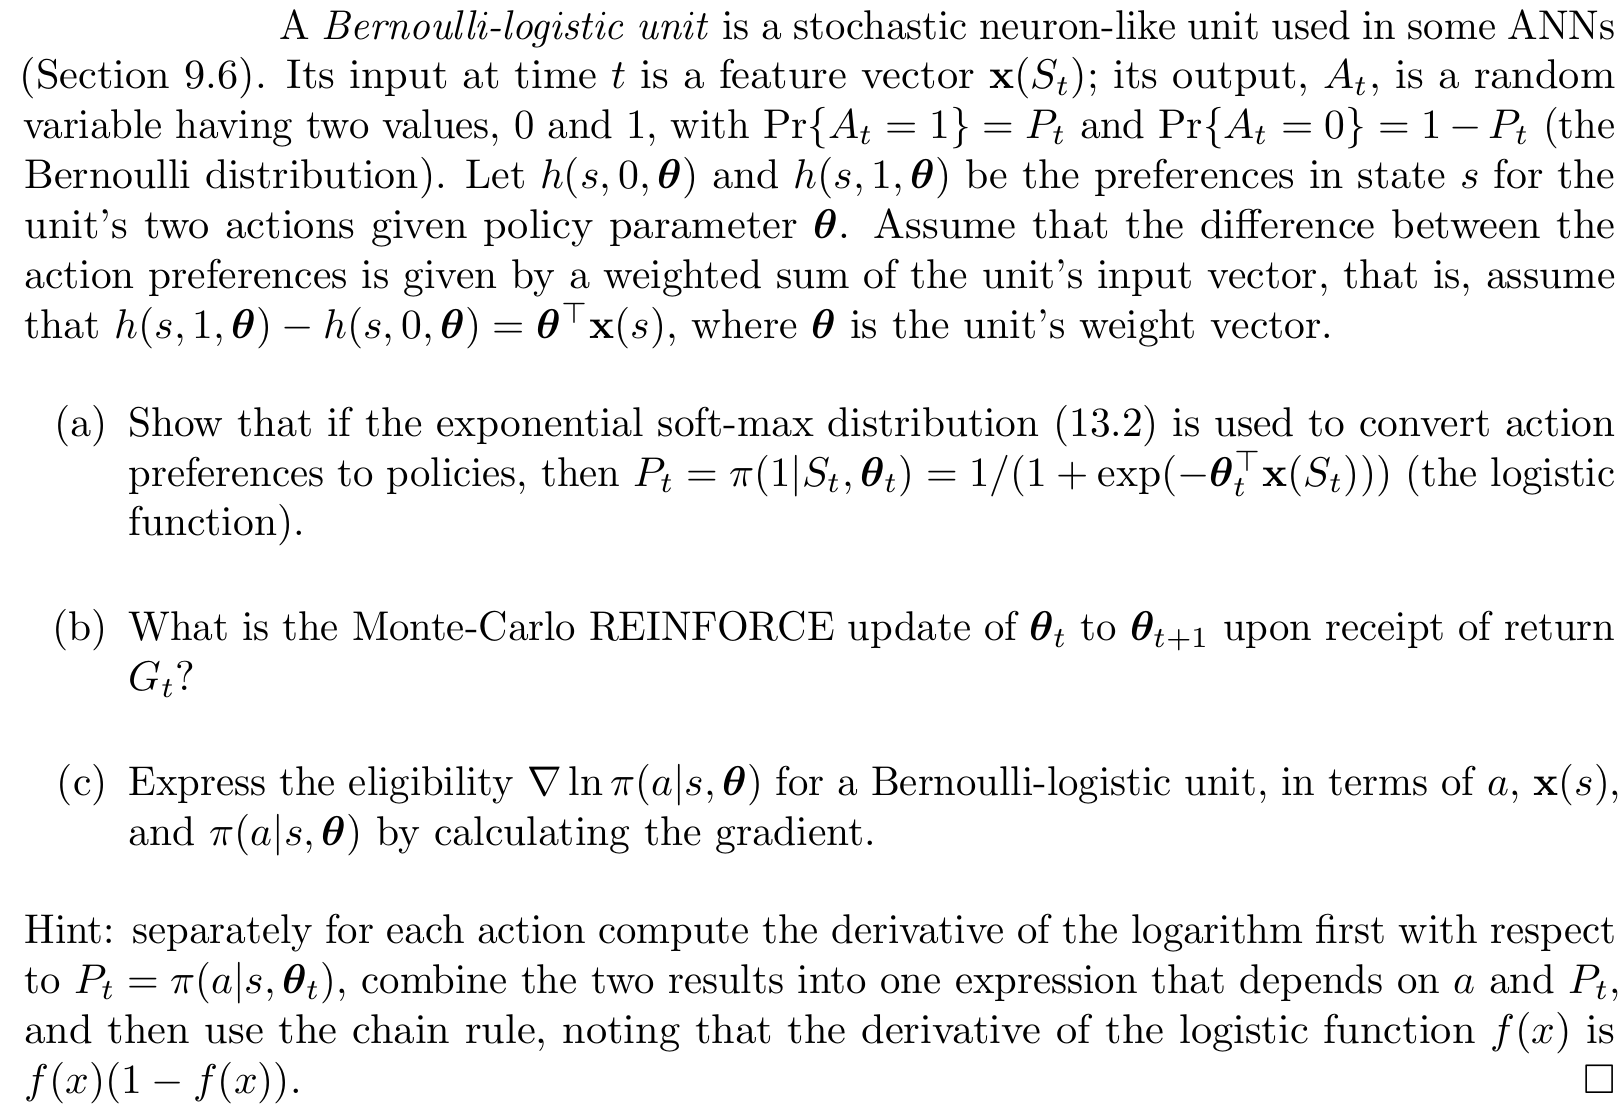
\includegraphics[scale=0.9]{exercise_13_5q}

    \subsection*{Answer}

    \subsubsection*{a}

    \noindent $ \pi(s, 1, \theta) = \frac{e^{h(s,1, \theta)}}{e^{h(s,1, \theta)} + e^{h(s,0, \theta)}} $

    \noindent $ \pi(s, 1, \theta) = \frac{e^{h(s,1, \theta)}}{e^{h(s,1, \theta)} + e^{h(s,1, \theta)-\theta x(s)}} $

    \noindent $ \pi(s, 1, \theta) = \frac{1}{1 + e^{-\theta x(s)}} $

    \subsubsection*{b}

    \noindent $ \theta_{t+1} = \theta_t + \alpha G_t \nabla \ln \pi(A_t | S_t, \theta_t) $ \hfill From equation 13.8

    \subsubsection*{c}

    I am not sure about the result.
    I followed the steps hoping to reach a reasonable result.
    The result I found seems be reasonable but it does not include the x(s) term.

    \hfill \break
    \noindent Separately for each action computing the derivative of the logarithm with respect to P

    \hfill \break
    \noindent $  \pi(1 | S_t, \theta_t) = P_t$

    \noindent $  \ln \pi(1 | S_t, \theta_t) = \ln P_t$

    \noindent $  \nabla \ln \pi(1 | S_t, \theta_t) = \frac{P_t^'}{P_t} = \frac{P_t (1-P_t)}{P_t} = 1-P_t  $

    \hfill \break
    \noindent $  \pi(0 | S_t, \theta_t) = 1- P_t$

    \noindent $  \ln \pi(0 | S_t, \theta_t) = \ln (1- P_t)$

    \noindent $  \nabla \ln \pi(0 | S_t, \theta_t) = \frac{P_t^'}{1-P_t} = \frac{P_t (1-P_t)}{1-P_t} = P_t  $

    \hfill \break
    \noindent Combining both results into one expressing that depends on a and P

    \noindent $  \nabla \ln \pi(a | S_t, \theta_t) = a \nabla \ln \pi(1 | S_t, \theta_t) + (1-a) \nabla \ln \pi(0 | S_t, \theta_t)  $

    \noindent $  \nabla \ln \pi(a | S_t, \theta_t) = a (1- P_t) + (1-a) P_t  $

    \hfill \break
    \noindent Now replacing with P with $\pi$ and rearranging:

    \noindent $  \nabla \ln \pi(a | S_t, \theta_t) = a \pi(0 | S_t, \theta_t) + (1-a) \pi(1 | S_t, \theta_t)  $

    \noindent $  \nabla \ln \pi(a | S_t, \theta_t) = a (1 - \pi(1 | S_t, \theta_t)) + (1-a) (1- \pi(0 | S_t, \theta_t))  $

    \hfill \break
    \noindent The first part is non-zero only when a is 1.
    The second part is only non-zero only when a is 0.
    Thus we can replace selected actions with a:

    \noindent $  \nabla \ln \pi(a | S_t, \theta_t) = a (1 - \pi(a | S_t, \theta_t)) + (1-a) (1- \pi(a | S_t, \theta_t))  $

    \noindent $  \nabla \ln \pi(a | S_t, \theta_t) = 1- \pi(a | S_t, \theta_t) $


\end{document}


